%%%%%%%% CS-502 EXAMPLE LATEX SUBMISSION FILE %%%%%%%%%%%%%%%%%

\documentclass{article}

% Recommended, but optional, packages for figures and better typesetting:
\usepackage{microtype}
\usepackage{graphicx}
\usepackage{subfigure}
\usepackage{booktabs} % for professional tables
\usepackage{hyperref}

\usepackage[accepted]{cs502}

\icmltitlerunning{Submission and Formatting Instructions for ICML 2021}

\begin{document}

\twocolumn[
\icmltitle{CS 502 - Project report}

\begin{icmlauthorlist}
\icmlauthor{Member 1}{}
\icmlauthor{Member 2}{}
\icmlauthor{Member 3}{}
\end{icmlauthorlist}

\vskip 0.3in
]

\begin{abstract}
Put your abstract here.
\end{abstract}

\section{Introduction}

This Latex template is adapted from the ICML template.

\section{Method}

\section{Experiments}

\section{Conclusion}

\section{Others}

\subsection{Example of adding figure}

\begin{figure}[ht]
\vskip 0.2in
\begin{center}
\centerline{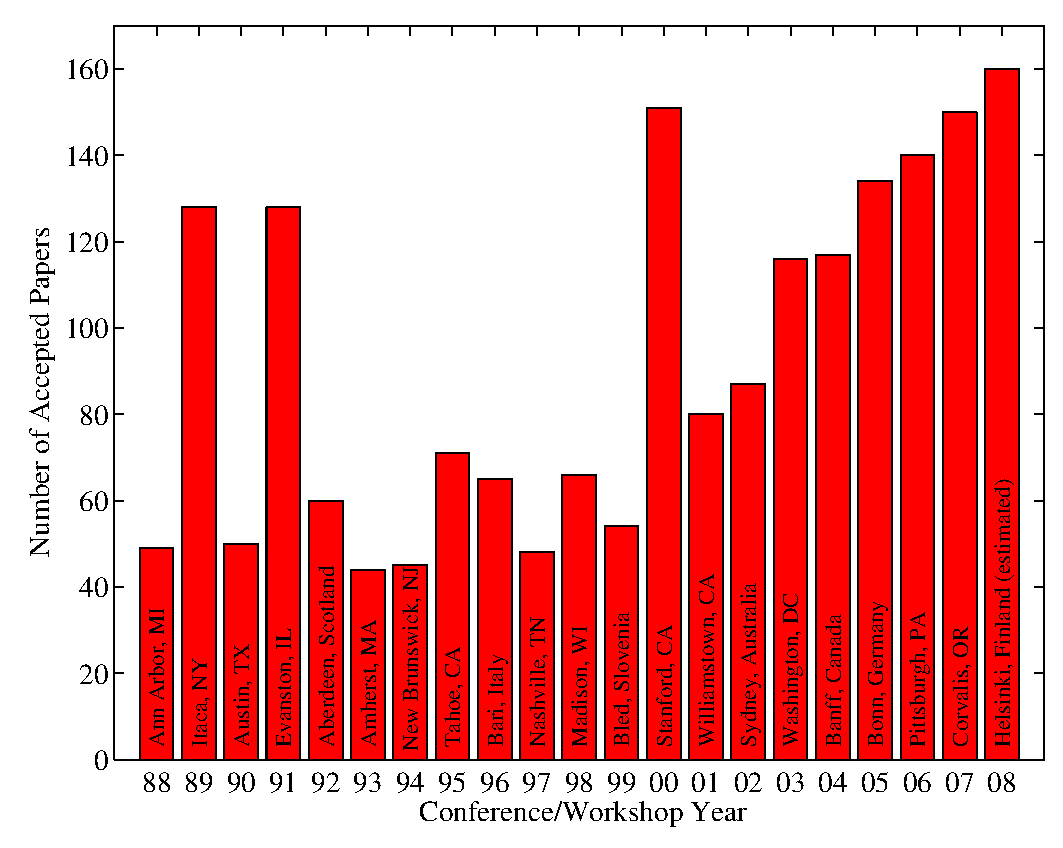
\includegraphics[width=0.85\columnwidth]{example}}
\caption{Example figure}
\label{example}
\end{center}
\vskip -0.2in
\end{figure}

\subsection{Example of adding table}

\begin{table}[h]
\caption{Example table}
\label{sample-table}
\vskip 0.15in
\begin{center}
\begin{small}
\begin{sc}
\begin{tabular}{lcccr}
\toprule
Data set & Naive & Flexible & Better? \\
\midrule
Breast    & 95.9$\pm$ 0.2& 96.7$\pm$ 0.2& $\surd$ \\
Cleveland & 83.3$\pm$ 0.6& 80.0$\pm$ 0.6& $\times$\\
Glass2    & 61.9$\pm$ 1.4& 83.8$\pm$ 0.7& $\surd$ \\
Credit    & 74.8$\pm$ 0.5& 78.3$\pm$ 0.6&         \\
\bottomrule
\end{tabular}
\end{sc}
\end{small}
\end{center}
\vskip -0.1in
\end{table}


\subsection{Example of adding reference}

Paper \cite{example}.


\bibliography{main}
\bibliographystyle{cs502}

\end{document}

